\chapter{Methodology for extracting and filtering logical dependencies}
\label{extraction}

\section{Overview of the approach}
\label{sec:overview_approach}
To be done at the end


\section{Data collection}
\label{sec:data_collection}


\subsection{Data set used}
\label{subsec:data_sets_used}

\hspace{4em}To investigate logical dependencies extraction and filtering techniques and their interplay with structural dependencies, 27 open-source projects from GitHub\footnote{http://github.com/} were selected. Table \ref{table:1} provides an overview of all the software systems analyzed.

The table consists of five columns: the \textit{ID} column assigns a unique identifier to each project. The \textit{Project name} column lists the project names as they appear on GitHub. The \textit{Number of entities} column specifies the total number of entities (classes and interfaces) extracted from the source code. The \textit{Number of commits} column specifies the number of commits analyzed from the active branch (main/master) of each project. Lastly, the \textit{Type} column specifies the programming language in which the project was developed.

This selection includes projects implemented in two programming languages: Java and C\#. The systems vary in size and complexity. From a structural perspective, the smallest project is \textit{shipkit}, which contains only 639 entities, while the largest is \textit{EntityFrameworkCore}, with 50,179 entities.

Regarding commit history, \textit{shipkit} is again the smallest, with 1,563 commits analyzed, while \textit{aeron} is the largest, with 5,977 commits. This selection of projects allows a better investigation of how filtering techniques affect systems of different sizes and commit histories.


\begin{table}[!h]
\renewcommand{\arraystretch}{1}
\caption{Summary of open source projects used for logical dependencies extraction and filtering.}
\label{table:1}
\centering
\scalebox{0.9}{
\begin{tabular}{|c|c|c|c|c|c|}
\hline
   ID  & Project name   & Number of & Number of& Type\\
     &     & entites & commits & \\
\hline
1	&	bluecove	&	2685	&	894	&	Java	\\
2	&	aima-java	&	5232	&	1006	&	Java	\\
3	&	powermock	&	2801	&	949	&	Java	\\
4	&	restfb	&	3350	&	1391	&	Java	\\
5	&	rxjava	&	21097	&	4398	&	Java	\\
6	&	metro-jax-ws	&	6482	&	2927	&	Java	\\
7	&	mockito	&	5189	&	3330	&	Java	\\
8	&	grizzly	&	10687	&	3113	&	Java	\\
9	&	shipkit	&	639	&	1563	&	Java	\\
10	&	OpenClinica	&	9655	&	3276	&	Java	\\
11	&	robolectric	&	8922	&	5912	&	Java	\\
12	&	aeron	&	4159	&	5977	&	Java	\\
13	&	antlr4	&	4747	&	4431	&	Java	\\
14	&	mcidasv	&	3272	&	4136	&	Java	\\
15	&	ShareX	&	4289	&	5485	&	C\#	\\
16	&	aspnetboilerplate	&	9712	&	4323	&	C\#	\\
17	&	orleans	&	16963	&	3995	&	C\#	\\
18	&	cli	&	2063	&	4488	&	C\#	\\
19	&	cake	&	12260	&	2518	&	C\#	\\
20	&	Avalonia	&	16732	&	5264	&	C\#	\\
21	&	EntityFrameworkCore	&	50179	&	5210	&	C\#	\\
22	&	jellyfin	&	8764	&	5433	&	C\#	\\
23	&	PowerShell	&	2405	&	3250	&	C\#	\\
24	&	WeiXinMPSDK	&	7075	&	5729	&	C\#	\\
25	&	ArchiSteamFarm	&	702	&	2497	&	C\#	\\
26	&	VisualStudio	&	4869	&	5039	&	C\#	\\
27	&	CppSharp	&	17060	&	4522	&	C\#	\\
\hline
\end{tabular}
}
\end{table}




\subsection{Extracting structural dependencies}
\label{subsec:extracting_structural_dependencies}

\hspace{4em}A dependency is created between two elements that are in a relationship, indicating that one element of the relationship, in some manner, depends on the other \cite{Booch:2004:OAD:975416}, \cite{Cataldo2009SoftwareDW}.

Structural dependencies can be identified by analyzing the source code \cite{structdep}. A structural dependency between two entities (e.g., a class and an interface) exists if one entity statically depends on the other, meaning it cannot be compiled without the dependent entity. In object-oriented systems, this dependency can be given by various types of relationships: one entity extends another (for classes), implements another (for interfaces), has attributes of the other entity's type, has methods with the other entity's type in their signature, uses local variables of the other entity's type, or calls methods of the other entity \cite{Sangal:2005:UDM:1094811.1094824, CalloArias2011, 1199197}.

We use an external tool called \textit{srcML} \cite{srcML} to convert all source code files into XML files. We then extract all information about classes, interfaces, methods, or calls to other classes by parsing the XML files and building a dependency data structure. 

Maletic and Collard \cite{srcMLCollard, Collard:2011:LTF:2067850.2068011, CollardsrcML2005} developed the \textit{srcML} tool to offer an XML-based representation of the source code. The tool preserves all source code information, including comments and formatting. The tool supports languages such as C, C++, Java, and C\#, and provides command-line utilities for converting an entire project to and from the \textit{srcML} format. 

Another advantage of the \textit{srcML} tool is that it uses consistent markup for different programming languages, making it easier to extract structural dependencies from source code written in languages like Java, C++, Python, or C\#.



\subsection{Extracting Logical Dependencies}
\label{subsec:extracting_logical_dependencies}

\hspace{4em}\textit{Logical dependencies} (logical couplings) can be identified through software history analysis. Version control repositories (such as Git) store not only the source code of the system but also its change history. By examining both, we can extract structural and logical dependencies. The source code structure provides \textit{structural dependencies}, while the system’s change history reveals \textit{logical dependencies} formed by pairs of files or components that co-evolve.

As illustrated in Figure~\ref{fig:extracting_data_with_git}, the \texttt{git clone} command retrieves the entire repository, including its code and commit history. The \texttt{git diff} command then highlights differences between two specific commits, generating a text file that contains the differences between the two commits: code differences, the number of files changed, and the names of changed files.

\begin{figure}[H]
\centering
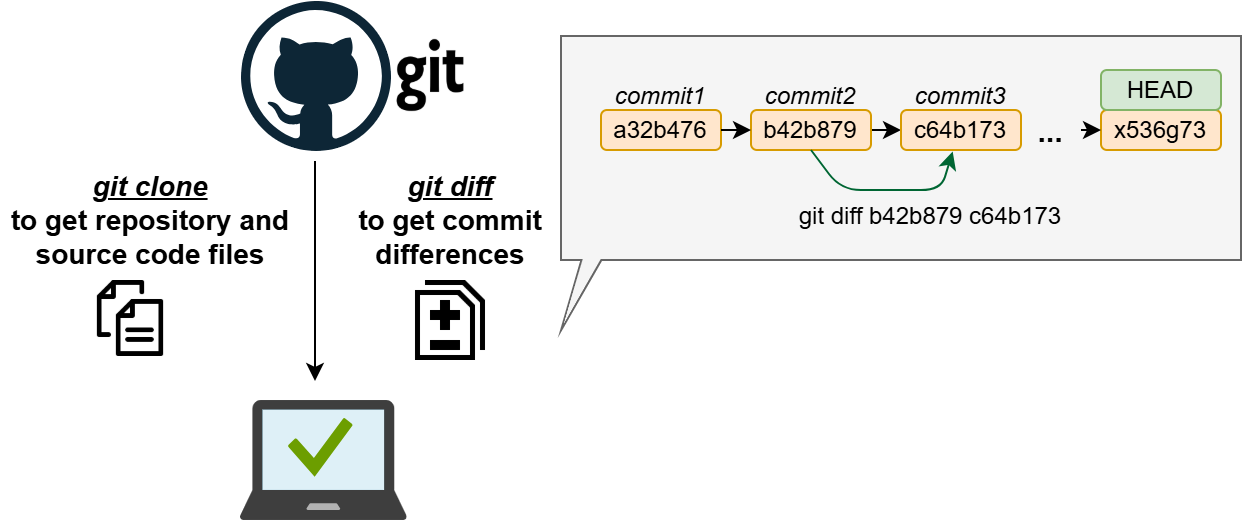
\includegraphics[width=\textwidth]{gitdata.png}
\caption{Using Git commands (\texttt{clone} and \texttt{diff}) to retrieve source code and commit changes.}
\label{fig:extracting_data_with_git}
\end{figure}


Listing \ref{lst:git_diff} provides an example of a \texttt{git diff} output for three files: \texttt{User.java}, \texttt{Calculator.java}, and \texttt{Utils.java}. From the diff output, we can identify the names of the changed files and information about added or deleted lines of code, but not the specific entities (e.g., classes or interfaces) from those files. 

To determine the changed entities, we first extract the structural dependencies of the system and create a mapping between the entities defined in each file and the file. Later, we associate the changed files with their corresponding entities when processing the diff files using this mapping \cite{DepSACI, b4, icstcc-2024, enase19}. 

For instance, in this example, the mapping can reveal that \texttt{User.java} contains the class \texttt{User}, \texttt{Calculator.java} contains the class \texttt{Calculator}, and \texttt{Utils.java} contains the class \texttt{Utils}. Even if Java typically enforces a standardized relationship between file and entity names, this is not always the case for other programming languages, so we need a uniform approach.

Using this mapping, we can say that the commit presented in Listing \ref{lst:git_diff} generates three pairs of co-changed entities: \texttt{Utils-Calculator}, \texttt{Utils-User}, and \texttt{Calculator-User}.

\begin{lstlisting}[language=diff, caption={Example output of \texttt{git diff} between two commits.}, label={lst:git_diff}]
commit 1a2b3c4d5e (HEAD -> main)
Author: Developer <developer@example.com>
Date:   Wed Dec 13 12:34:56 2024 +0000

    Refactored code and added new features.

diff --git a/src/User.java b/src/User.java
index abc1234..def5678 100644
--- a/src/User.java
+++ b/src/User.java
@@ -1,5 +1,6 @@
+    public User(String name) {
+        this.name = name;
+    }

-    public void greet() {
+    public void displayGreeting() {
         System.out.println("Hello, " + name + "!");
     }
 }

diff --git a/src/Calculator.java b/src/Calculator.java
index 9876543..2345678 100644
--- a/src/Calculator.java
+++ b/src/Calculator.java
@@ -5,7 +5,7 @@ 
-    public int subtract(int a, int b) {
+    public int subtractNumbers(int a, int b) {
         return a - b;
     }
 }

diff --git a/src/Utils.java b/src/Utils.java
index 56789ab..789abcd 100644
--- a/src/Utils.java
+++ b/src/Utils.java
@@ -3,7 +3,7 @
-    public static String getCurrentTime() {
+    public static String getFormattedTime() {
         return java.time.LocalTime.now().toString();
     }
 }
\end{lstlisting}




\section{Tool for measuring software dependencies}
\label{subsec:tool_measuring_dependencies}

\hspace{4em}To extract structural and logical dependencies, we developed a tool that takes as input the source code repository URL of a given system and extracts the corresponding software dependencies \cite{DepSACI, enase19}. 

From a workflow perspective, the tool performs three main activities: downloading the necessary data from the repository, extracting structural dependencies from the source code, and identifying and filtering co-changing pairs from the repository's commit history. Figure \ref{fig:figworkflow} illustrates these activities, with each block representing a different step from the process.


To get the source code files and the change history, we first need to know the repository URL from GitHub (GitHub is a Git repository cloud-based hosting service). With the GitHub URL and a series of Git commands, the tool can download all the necessary data for dependencies extraction.


As presented in figure \ref{fig:extracting_data_with_git}, the \textit{"git clone"} command will download a repository, including the source code files. The \textit{"git diff"} command will get the differences between two existing commits in the Git repository. 
The tool gets the Git repository and the source code files by executing the "clone" command. Afterward, it gets all the existing commits within the Git repository. The commits are ordered by date, beginning with the oldest one and ending with the most recent one. The tool executes the "diff" command between each commit and its parent (the previous commit). The "diff" command generates a text file that contains the differences between the two commits: code differences, the number of files changed and changed file names.


The first step involves downloading the source code files and change history. This requires the GitHub repository URL, as GitHub is a cloud-based hosting service for Git repositories. Using this URL and Git commands, the tool downloads all the data necessary for dependency extraction.

\begin{figure}[H]
\centering
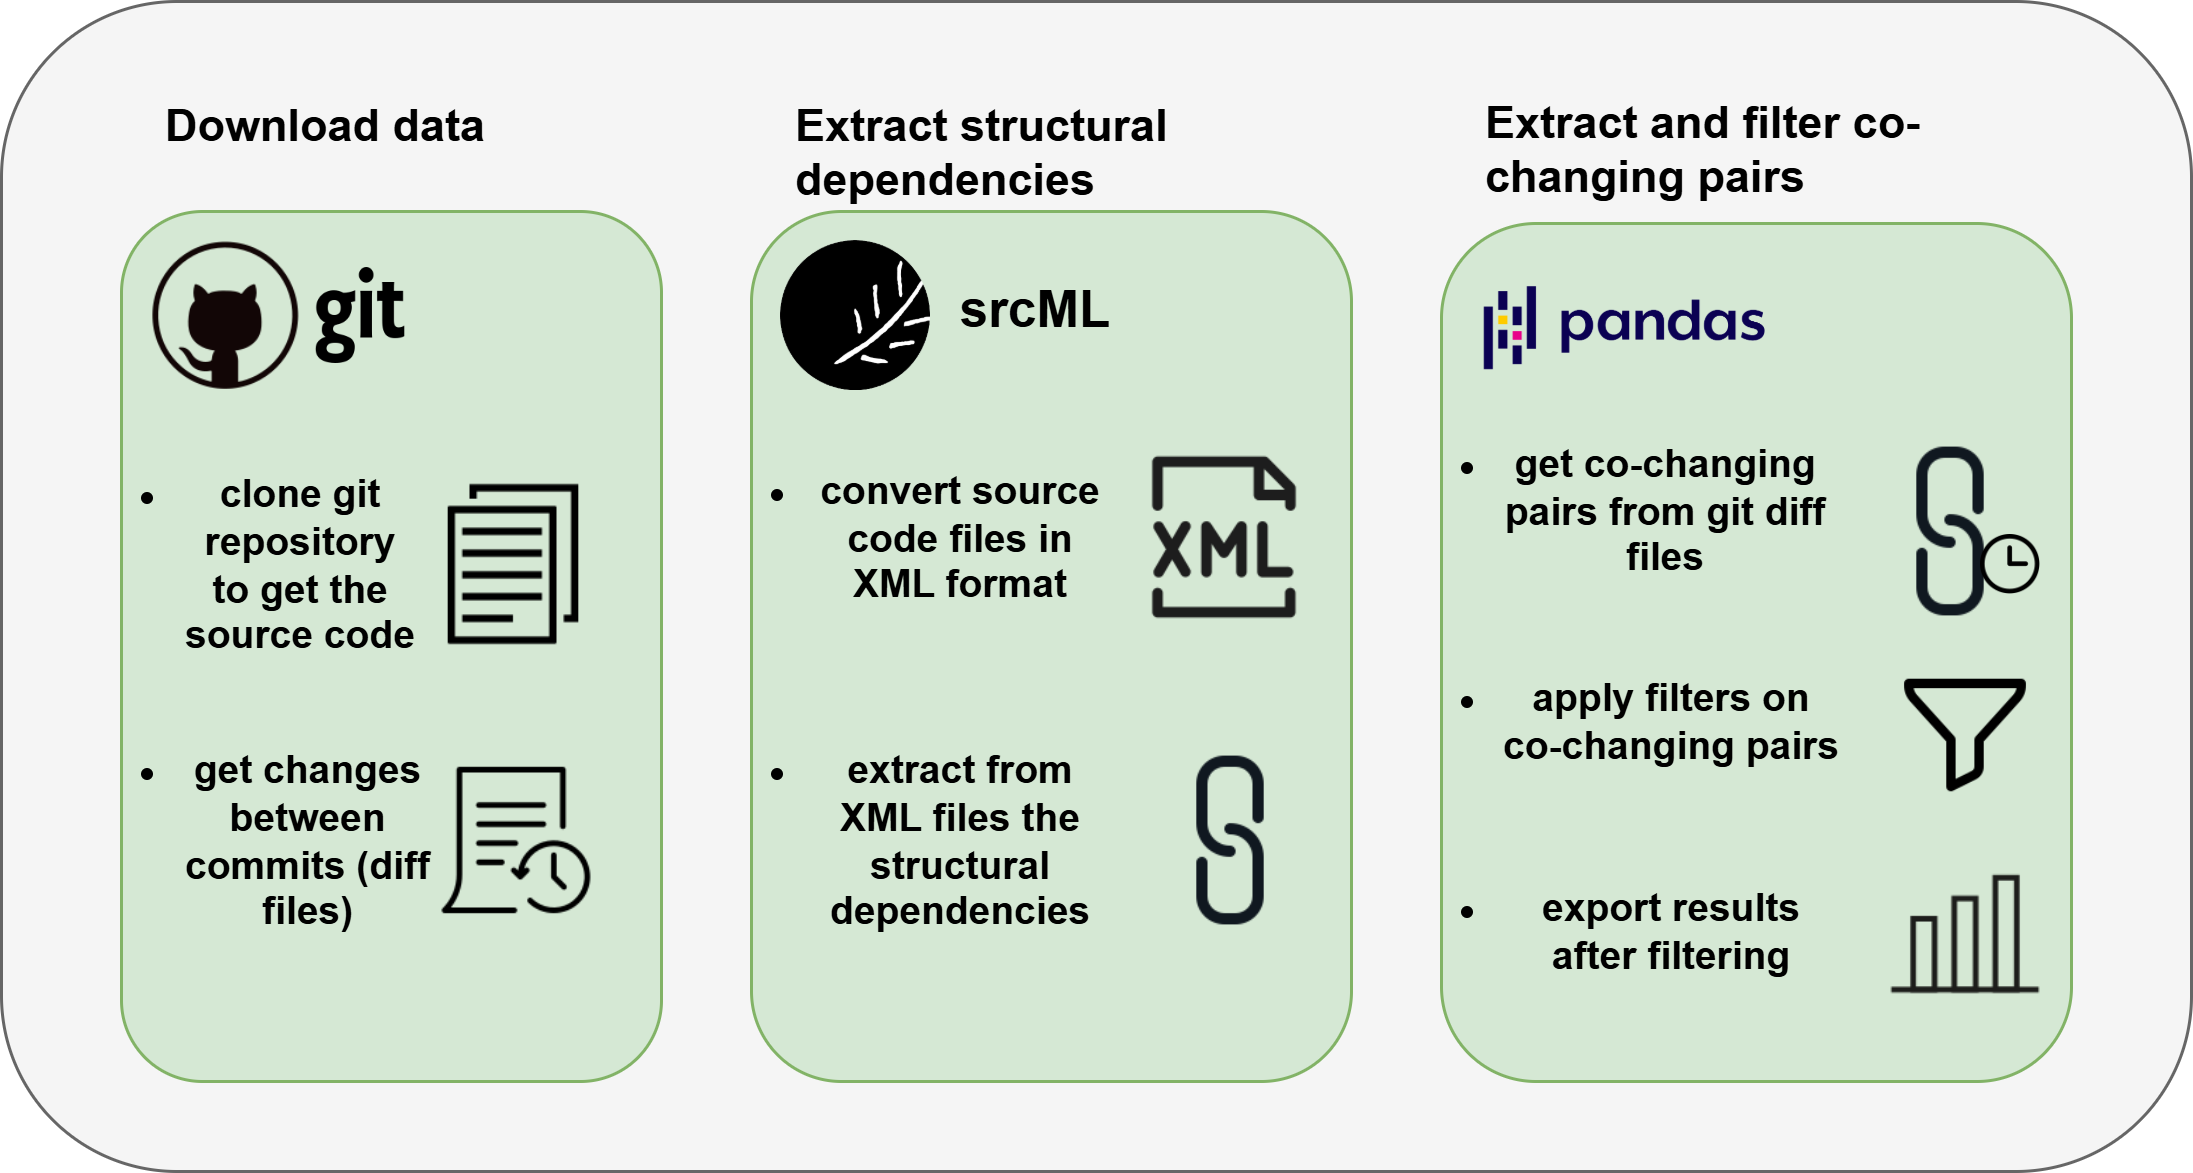
\includegraphics[width=\textwidth]{tool_workflow.png}
\caption{Tool workflow and major activities.}
\label{fig:figworkflow}
\end{figure}



\textbf{Extract structural dependencies.}

To extract structural dependencies from the source code, the tool first converts each source file into the srcML format using the method introduced in subsection \ref{subsec:extracting_structural_dependencies}. The srcML format provides an XML representation of the source code, with markup tags identifying elements of the programming language syntax\cite{srcML}. 

Once converted, the tool parses each file to identify all defined entities (such as classes, interfaces, and enums) from the file. It also detects all entities used by the defined entities. The connections between the defined and used entities form the structural dependencies.


\textbf{Extract and filter co-changing pairs.}

The process of extracting and filtering co-changing pairs is illustrated in Figure \ref{fig:figfiltering}.

To analyze the changes between commits, the tool uses the \texttt{"git diff"} command. All existing commits in the repository are collected and chronologically ordered, starting with the oldest and ending with the most recent. For each commit, the tool runs the \texttt{"git diff"} command to compare it with its parent (the preceding commit). This generates a text file containing the details of the changes between the two commits.

To extract co-changing pairs, the tool parses each generated diff file. From each file, it identifies the number of changed files and their names. Since the tool already knows the software entities contained in each file (from the structural dependencies extraction), it can determine co-changing pairs by linking entities from changed files. Once all the co-changing pairs for a diff file are extracted, the tool moves to the next diff file and repeats the process.

Explained in more detail in subsections \ref{subsec:filtering_transaction_size}, \ref{subsec:filtering_support}, and \ref{subsec:filtering_connection_strength}, not every extracted co-changing pair is considered a logical dependency. For a pair to be considered a logical dependency, it must pass some criteria. These criteria are implemented as filters in the tool. Each filter processes the extracted co-changing pairs and outputs the pairs that meet the filter requirements. The filters can also be combined to ensure that only meaningful logical dependencies remain after filtering.

\begin{figure}[H]
\centering
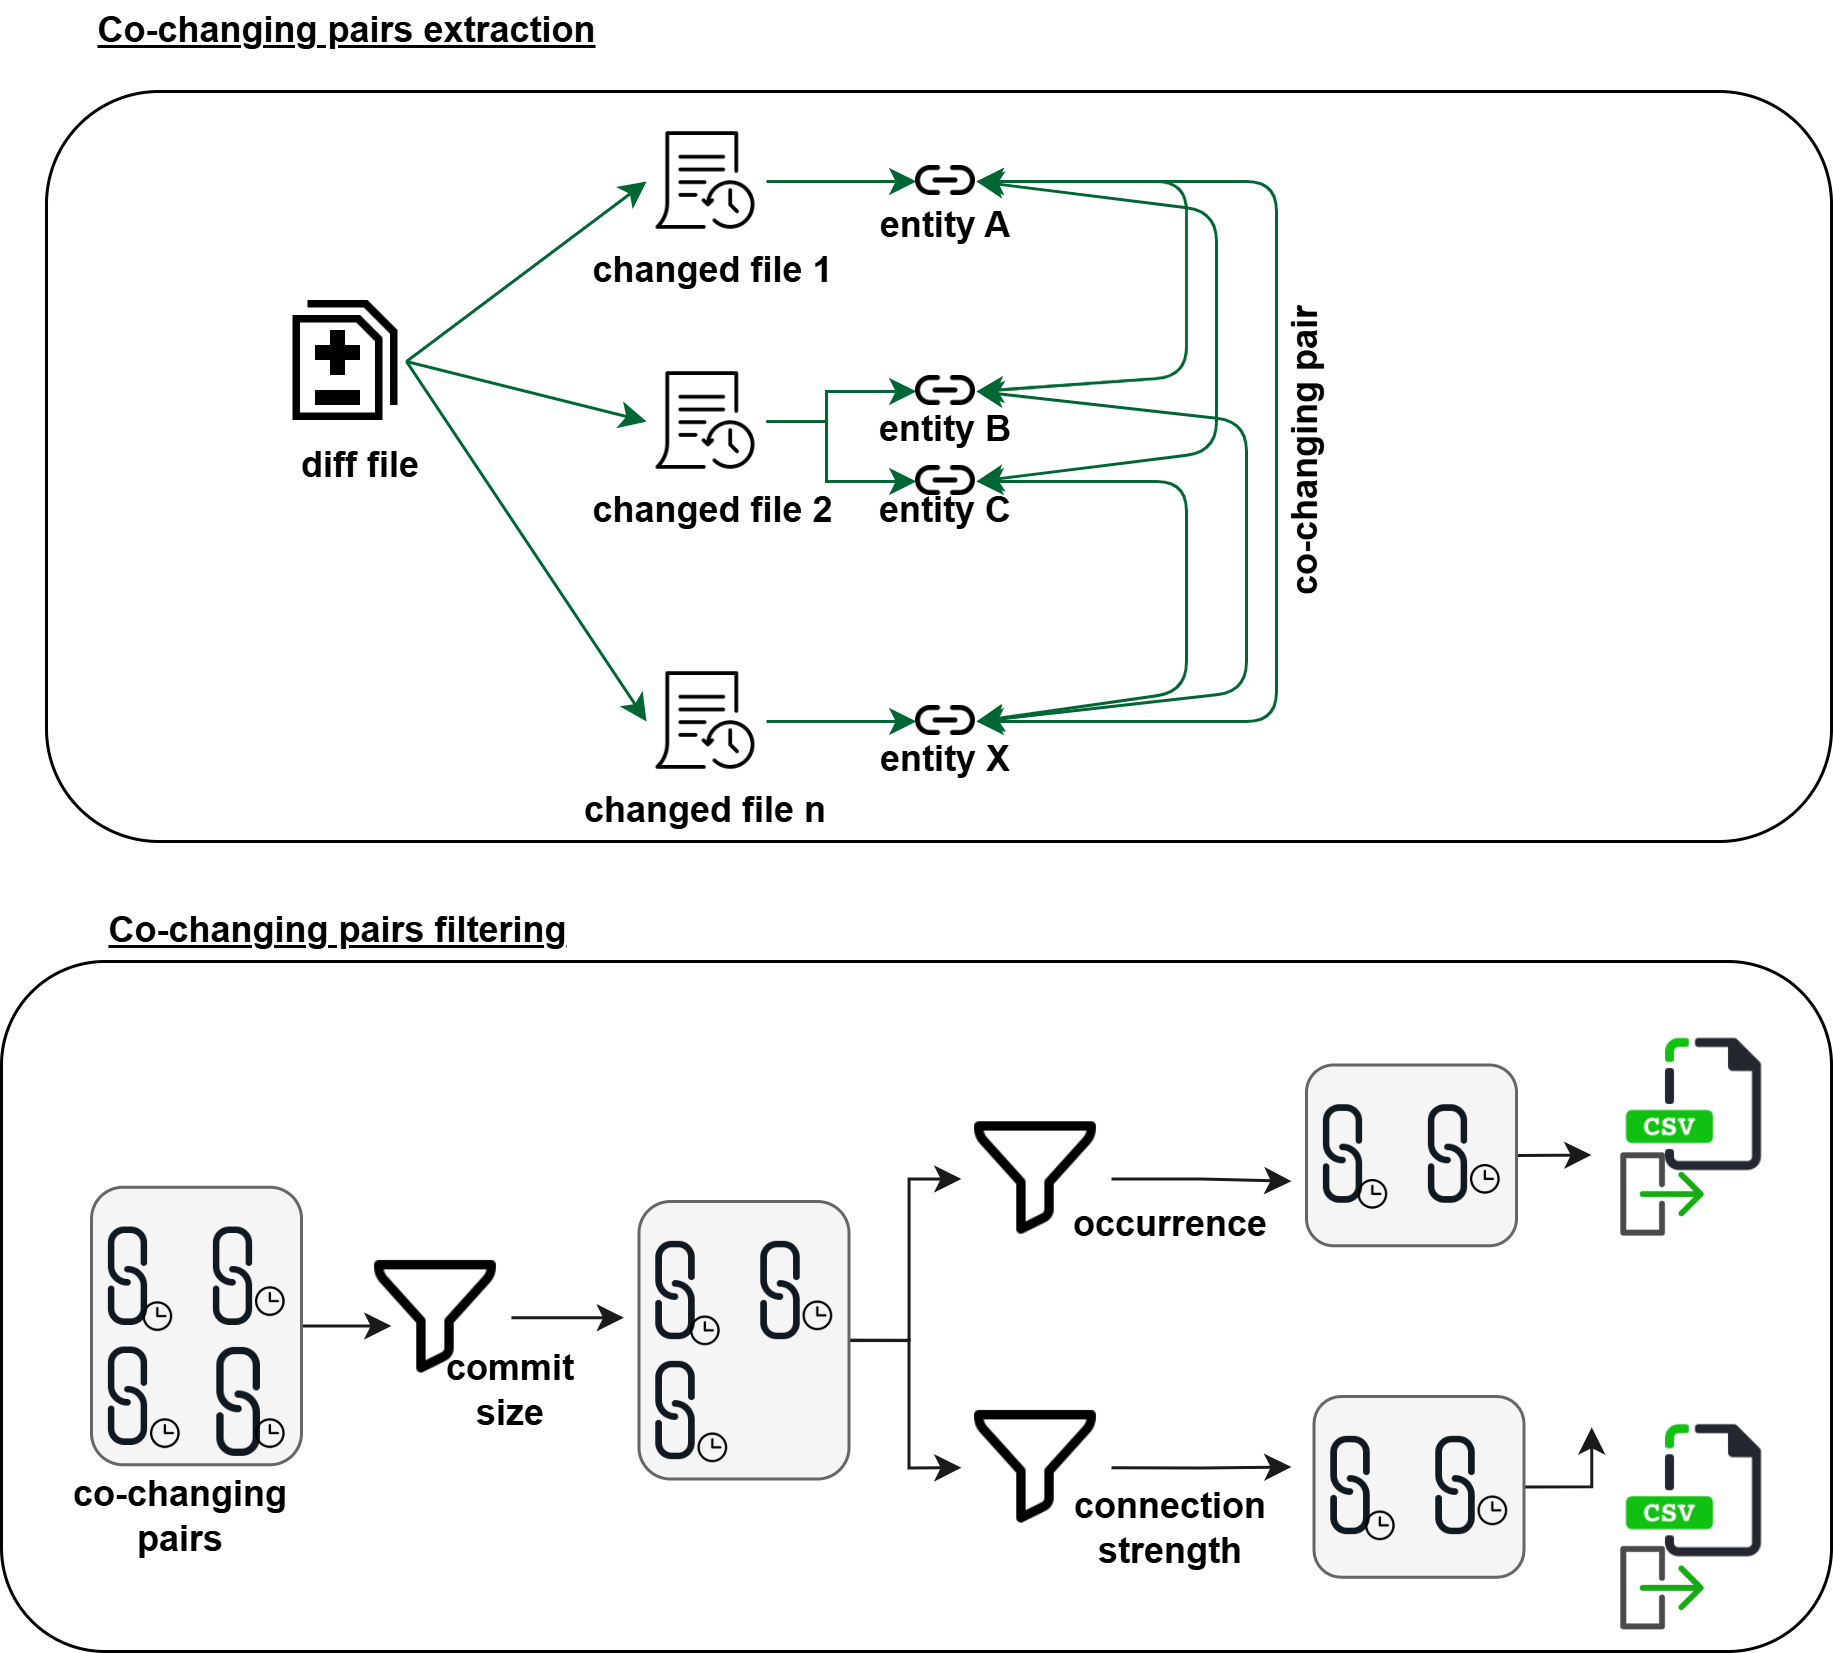
\includegraphics[width=\textwidth]{pairs_filtering.png}
\caption{Co-changing pairs extraction and filtering.}
\label{fig:figfiltering}
\end{figure}



\section{Filtering logical dependencies}
\label{sec:filtering_logical_dependencies}

\hspace{4em}As discussed in Section \ref{ld-intro}, the number of co-changing pairs extracted from software repositories can be quite large, often reaching millions. This quantity, combined with noise in the data, makes it important to apply filtering techniques to identify meaningful co-changing pairs.

This section presents three filtering techniques used to refine the extracted co-changing pairs. The filter based on commit transaction size, discussed in Section \ref{subsec:filtering_transaction_size}, is always applied. The experiments are performed by combining this filter with one of the other two filters: the support filter presented in Section \ref{subsec:filtering_support} or the connection strength filter discussed in Section \ref{subsec:filtering_connection_strength}. The commit size filter aims to reduce the overall size of the co-changing pairs, while the support and connection strength filters aim to minimize noise in the data.

\subsection{Filtering based on commit transaction size}
\label{subsec:filtering_transaction_size}

As discussed in Section \ref{ld-intro}, the number of co-changing pairs extracted from software repositories can be quite large, often reaching millions. 

With this filtering approach, the goal is to reduce the total number of extracted co-changing pairs and move closer to identifying meaningful logical dependencies. With the filter based on commit size (\textit{cs}), only co-changing pairs from commits involving fewer files than a predefined threshold are considered.

Large commits, which often involve numerous files, are usually because of non-functional changes, such as branch merges, folder restructuring, or formatting updates. These types of commits can introduce noise by creating irrelevant co-changing pairs.

Different studies have used various threshold values for filtering commit sizes. Cappiluppi and Ajienka \cite{DBLP:journals/jss/AjienkaC17, DBLP:journals/ese/AjienkaCC18} only considered commits with fewer than 10 modified source code files. Similarly, Kagdi et al. used the same threshold, excluding commits with more than 10 source files. Ying et al. \cite{Ying-co-change} took a different approach, excluding commits involving over 100 files. Zimmermann et al. \cite{Zimmermann:2004:MVH:998675.999460} configured the ROSE tool to exclude commits larger than 30 files. Moonen et al. \cite{Moonen-commit} explored seven different transaction filtering sizes (2, 4, 6, 8, 10, 20, and 30), recommending a threshold of 8 files.



We analyzed the overall transaction size trend for 27 open-source C\# and Java systems with a total of 74,332 commits. The results are presented in Figure \ref{fig:fig_cs} and in Table \ref{table:cs_values}. Based on the analysis, we observed that 90\% of the total commit transactions involved fewer than 10 source code files. This percentage indicates that setting a threshold of 10 files for the maximum size of commit transactions will not affect too much the total number of commits available for extracting co-changing pairs, 90\% of the transactions still remain available for analysis \cite{DepSACI, enase19}.

Table \ref{table:cs_values} provides more details of the commit transaction size distribution for each system. The columns in the table represent the following information:

\hspace{-4em}- \textit{$cs\leq 5$}: The number of commits with a transaction size of 5 or fewer files. \\
- \textit{$cs\leq 10$}: The number of commits with a transaction size of 10 or fewer files. \\
- \textit{$cs\leq 20$}: The number of commits with a transaction size of 20 or fewer files. \\
- \textit{$cs<\infty$}: The total number of commits for the system. \\
- \textit{$Avg$}: The average transaction size for the system.


\begin{figure}[!h]
\centering
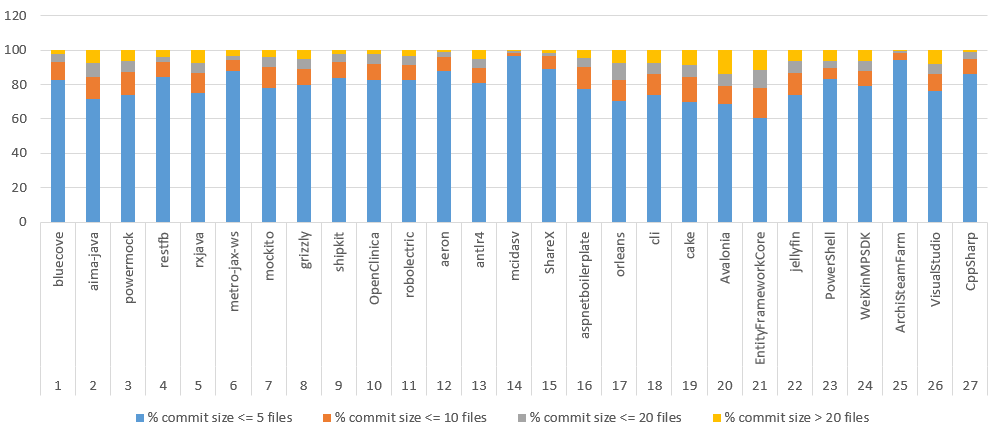
\includegraphics[width=\textwidth]{commit_distribution.png}
\caption{Commit transaction size(cs) trend in percentages.}
\label{fig:fig_cs}
\centering
\end{figure}


\begin{figure}[!h]
\centering
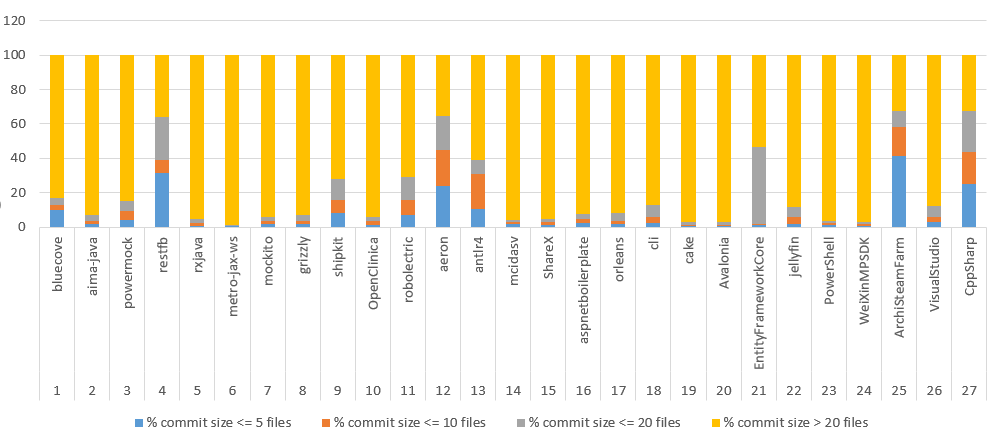
\includegraphics[width=\textwidth]{ld_distribution.png}
\caption{Percentages of co-changing pairs extracted from each commit transaction size(cs) group.}
\label{fig:fig_ld_cs}
\centering
\end{figure}

As we can see in Figure \ref{fig:fig_ld_cs}, even though only 5\% of the commit transactions have more than 20 files changed ($20<cs<\infty$), they generate, on average, 80\% of the total amount of co-changing pairs extracted from the systems.  
The high number of co-changing pairs extracted from such a small number of commit transactions is caused by the number of files involved in those commit transactions.  

One single commit transaction can lead to a large amount of co-changing pairs. For example, in RxJava, we have commit transactions with 1030 source code files. This means that those commits can generate  
\[
\Comb{n}{k}=\frac{n!}{k!(n-k)!} = \frac{1030!}{2!(1028)!} = 529 935
\]
logical dependencies. By setting a threshold on the commit transaction size, we can avoid the introduction of those co-changing pairs into the system.  

Filtering 10\% of the total amount of commit transactions can significantly decrease the number of co-changing pairs. That is why we choose the value of 10 files as our fixed threshold for the maximum size of a commit transaction \cite{DepSACI}.



\begin{table}[!h]
\renewcommand{\arraystretch}{1}
\caption{Commit transaction size(cs) trend and average per system.}
\label{table:cs_values}
\centering
\scalebox{0.9}{
\begin{tabular}{|c|c|c|c|c|c|c|}
\hline
$Nr.$	  & $Project $   &	$cs\leq 5$	&	$cs\leq 10$	&	$cs\leq 20$	&	$cs<\infty$ & Avg	\\ 
\hline
1	&	bluecove	&	738	&	97	&	37	&	22	&	4.9	\\
2	&	aima-java	&	733	&	134	&	74	&	65	&	7.24	\\
3	&	powermock	&	685	&	128	&	66	&	70	&	9.61	\\
4	&	restfb	&	1160	&	127	&	44	&	60	&	9.9	\\
5	&	rxjava	&	3395	&	447	&	253	&	303	&	8.46	\\
6	&	metro-jax-ws	&	2583	&	198	&	78	&	68	&	4.33	\\
7	&	mockito	&	2522	&	433	&	222	&	153	&	6.33	\\
8	&	grizzly	&	2487	&	302	&	180	&	144	&	5.28	\\
9	&	shipkit	&	1311	&	151	&	64	&	37	&	4.26	\\
10	&	OpenClinica	&	2837	&	250	&	119	&	70	&	3.31	\\
11	&	robolectric	&	4827	&	503	&	264	&	318	&	7.43	\\
12	&	aeron	&	4844	&	684	&	300	&	149	&	4.6	\\
13	&	antlr4	&	3426	&	437	&	304	&	264	&	8.5	\\
14	&	mcidasv	&	3996	&	81	&	35	&	24	&	2.47	\\
15	&	ShareX	&	4731	&	529	&	145	&	80	&	4.69	\\
16	&	aspnetboilerplate	&	3208	&	569	&	321	&	225	&	6.61	\\
17	&	orleans	&	2780	&	518	&	369	&	328	&	8.95	\\
18	&	cli	&	3377	&	551	&	308	&	252	&	6.43	\\
19	&	cake	&	1785	&	359	&	174	&	200	&	9.89	\\
20	&	Avalonia	&	3806	&	641	&	371	&	446	&	8.43	\\
21	&	EntityFrameworkCore	&	2866	&	878	&	644	&	822	&	15.38	\\
22	&	jellyfin	&	4007	&	662	&	419	&	345	&	6.25	\\
23	&	PowerShell	&	2702	&	224	&	133	&	191	&	7.33	\\
24	&	WeiXinMPSDK	&	4604	&	526	&	296	&	303	&	9.01	\\
25	&	ArchiSteamFarm	&	2357	&	92	&	28	&	20	&	2.24	\\
26	&	VisualStudio	&	3902	&	521	&	295	&	321	&	6.71	\\
27	&	CppSharp	&	3870	&	390	&	203	&	59	&	3.28	\\
\hline
\end{tabular}
}
\end{table}





\subsection{Filtering based on support}
\label{subsec:filtering_support}

\hspace{4em}In the previous section, we filtered the co-changing pairs based on commit size. Although this reduced the number of extracted co-changing pairs, this type of filtering does not guarantee that the remaining co-changing pairs are valid logical dependencies. A single occurrence of a co-changing pair could represent a valid logical dependency, but it could also be a coincidence.  

To address this, the \textit{support metric} is applied. The support metric of a rule $(A \rightarrow B)$, where $A$ is the antecedent and $B$ is the consequent, is defined as the number of commits (transactions) in which both entities are changed together. Many studies have used the support metric to filter logical dependencies. For example, \textit{Zimmermann et al.} \cite{Zimmermann:2004:MVH:998675.999460} applied minimum support thresholds of 1, 3, and 5 in their ROSE tool, while \textit{Kagdi et al.} \cite{article-Kagdi-commit} used thresholds of 1, 2, 4, and 8.

Considering only co-changing pairs with a minimum support threshold can help improve accuracy. However, for projects with a smaller number of commits, it becomes less likely to find co-changing pairs with high support, which could end up filtering out all the extracted co-changes.

We performed a series of analyses on the test systems, incrementing the support threshold (\textit{support}) from 1 to 4. Co-changing pairs were extracted only from commits with a transaction size of a maximum of 10 files. For each threshold mentioned above, the extracted co-changing pairs were then filtered based on the specified support threshold. Any co-changing pairs that did not meet the minimum support criteria were discarded.


Tables \ref{table:ld_ratio} and \ref{table:sd_percentages} provide detailed results for the support filtering applied to co-changing pairs. Table \ref{table:sd_percentages} presents the percentages of co-changing pairs that are also structural dependencies, and Table \ref{table:ld_ratio} presents the ratio of the number of co-changing pairs to the number of structural dependencies (SD). The columns in the tables represent the following information:

\hspace{-4em}- \textit{$Project\ nr.$}: The unique identifier assigned to each system. \\
- \textit{$support\geq 1$}: Represents the results when the minimum support threshold is set to 1, the ratio of co-changing pairs to structural dependencies (Table \ref{table:ld_ratio}) or the percentage of co-changing pairs that are also structural dependencies (Table \ref{table:sd_percentages}). \\
- \textit{$support\geq 2$}: Represents the results when the minimum support threshold is set to 2. \\
- \textit{$support\geq 3$}: Represents the results when the minimum support threshold is set to 3. \\
- \textit{$support\geq 4$}: Represents the results when the minimum support threshold is set to 4.


\begin{table}[!h]
\renewcommand{\arraystretch}{1}
\caption{Percentage of co-changing pairs that are also structural dependencies.}
\label{table:sd_percentages}
\centering
\scalebox{0.9}{
\begin{tabular}{|c|c|c|c|c|}
\hline
$Project\ nr.$ & $support\geq 1$ & $support\geq 2$ & $support\geq 3$ & $support\geq 4$  \\
\hline
1	&	7,13	&	7,77	&	7,99	&	19,71	\\
2	&	19,54	&	25,76	&	29,55	&	32,16	\\
3	&	6,66	&	8,58	&	11,82	&	14,87	\\
4	&	1,16	&	1,17	&	0,91	&	0,80	\\
5	&	3,99	&	3,96	&	7,75	&	7,49	\\
6	&	13,92	&	20,16	&	22,91	&	22,77	\\
7	&	8,38	&	9,28	&	14,93	&	14,58	\\
8	&	6,70	&	9,73	&	14,20	&	15,60	\\
9	&	16,98	&	23,34	&	29,22	&	32,89	\\
10	&	8,94	&	9,15	&	11,05	&	10,59	\\
11	&	4,99	&	6,92	&	8,88	&	11,08	\\
12	&	13,19	&	17,15	&	18,60	&	19,57	\\
13	&	2,43	&	5,59	&	8,33	&	8,21	\\
14	&	13,27	&	18,88	&	19,02	&	19,28	\\
15	&	12,90	&	21,95	&	25,51	&	27,01	\\
16	&	13,33	&	17,34	&	18,53	&	16,24	\\
17	&	6,09	&	6,18	&	6,41	&	6,44	\\
18	&	9,73	&	10,60	&	14,27	&	18,80	\\
19	&	10,26	&	13,54	&	13,64	&	12,60	\\
20	&	12,83	&	18,36	&	21,00	&	25,72	\\
21	&	2,86	&	4,65	&	5,70	&	4,98	\\
22	&	5,20	&	6,56	&	8,18	&	8,90	\\
23	&	8,23	&	13,64	&	17,04	&	17,65	\\
24	&	6,77	&	10,89	&	14,47	&	16,05	\\
25	&	9,85	&	10,15	&	11,65	&	11,33	\\
26	&	8,65	&	10,79	&	12,78	&	14,34	\\
27	&	7,04	&	8,78	&	9,87	&	10,08	\\
\hline
Avg	&	8,93	&	11,88	&	14,23	&	15,55	\\
\hline
\end{tabular}
}
\end{table}


\begin{table}[!h]
\renewcommand{\arraystretch}{1}
\caption{Ratio of number of co-changing pairs to number of structural dependencies. }
\label{table:ld_ratio}
\centering
\scalebox{0.9}{
\begin{tabular}{|c|c|c|c|c|}
\hline
$Project\ nr.$  & $support\geq 1$ & $support\geq 2$ & $support\geq 3$ & $support\geq 4$  \\
\hline
1	&	4,13	&	1,94	&	1,23	&	0,26	\\
2	&	0,81	&	0,33	&	0,16	&	0,10	\\
3	&	5,12	&	1,93	&	0,78	&	0,38	\\
4	&	53,36	&	42,00	&	38,31	&	36,30	\\
5	&	4,27	&	2,90	&	0,88	&	0,72	\\
6	&	1,07	&	0,46	&	0,30	&	0,23	\\
7	&	4,09	&	2,38	&	0,99	&	0,73	\\
8	&	4,06	&	1,57	&	0,76	&	0,49	\\
9	&	3,64	&	2,03	&	1,14	&	0,77	\\
10	&	1,41	&	1,01	&	0,47	&	0,34	\\
11	&	7,91	&	4,47	&	2,93	&	2,03	\\
12	&	3,92	&	2,15	&	1,47	&	1,07	\\
13	&	10,15	&	3,18	&	1,22	&	1,03	\\
14	&	3,07	&	1,53	&	1,16	&	0,97	\\
15	&	2,34	&	0,84	&	0,48	&	0,33	\\
16	&	1,21	&	0,47	&	0,26	&	0,19	\\
17	&	2,99	&	1,83	&	1,11	&	0,84	\\
18	&	2,26	&	1,37	&	0,67	&	0,40	\\
19	&	2,32	&	1,38	&	0,76	&	0,67	\\
20	&	1,24	&	0,58	&	0,35	&	0,18	\\
21	&	5,33	&	2,12	&	1,27	&	1,05	\\
22	&	3,38	&	1,88	&	0,99	&	0,74	\\
23	&	3,62	&	1,22	&	0,76	&	0,37	\\
24	&	2,57	&	1,22	&	0,67	&	0,46	\\
25	&	7,47	&	5,36	&	4,16	&	3,73	\\
26	&	4,03	&	2,16	&	1,50	&	1,15	\\
27	&	7,46	&	4,26	&	2,99	&	2,43	\\
\hline
Avg	&	5,67	&	3,43	&	2,51	&	2,15	\\
\hline
\end{tabular}
}
\end{table}
Based on Table \ref{table:sd_percentages}, we observe that only a small percentage of the extracted co-changing pairs overlap with structural dependencies. This observation is consistent with findings from related works \cite{DBLP:journals/jss/AjienkaC17, DBLP:journals/ese/AjienkaCC18}. The percentage of co-changing pairs that are structural dependencies increases as the minimum support threshold rises.

We calculate the overlap between co-changing pairs and structural dependencies not only to understand how many structural dependencies are reflected in the versioning system through co-changing pairs but also to filter out co-changing pairs that are structural dependencies, as they do not provide new information about the system.

We stopped the minimum support threshold at 4 because, as observed in Table \ref{table:ld_ratio}, systems with IDs 2, 6, 10, and 16 show a ratio below 1, indicating that the number of structural dependencies exceeds the number of co-changing pairs. For systems with IDs 4, 11, 25, and 27, increasing the threshold to 4 does not significantly reduce the difference between the number of co-changing pairs and structural dependencies.

Raising the support threshold beyond 4 risks filtering out all co-changing pairs for some systems. Therefore, while applying a threshold of 4 filters co-changing pairs to identify logical dependencies, the remaining number of co-changing pairs still significantly exceeds the number of structural dependencies for certain systems.




\subsection{Filtering based on connection strength}
\label{subsec:filtering_connection_strength}

